\section{Cisco CMX as IPS}
One of the companies that jumped on the bandwagon of the implementation of \acrlong{ips} is Cisco. Over the years they have developed a dashboard to gain intelligence from user's position such as hotspots where users gather most frequently and heat maps of different routes \acrlong{mu}s take. The definition provided by Cisco, states: ``Cisco’s CMX solution allows venues to simultaneously provide users with highly personalized content, provide services to customers to increase the customer experience, and gain visibility into customer behavior in their venues. CMX detects in-venue Wi-Fi enabled devices, prompts customers to connect to the wireless network, and engages them with value-added content and offers.`` \cite[p.~24]{Hallock2015}.
\subsection{Cisco MSE}
Cisco \acrfull{mse} is a platform that enables developers and users of this platform to centralize data, analyses and other \acrshort{wlan}-related statistics (e.g. coverage). Not only centralizing data but view the data is an important component of Cisco's \acrshort{mse}. Graphical plots such as heatmaps, interactive charts for user flows are part of this ecosystem (in CMX Analytics). It acts as the hardware engine behind the Cisco CMX technology, another option is to run the Cisco CMX platform on a dedicated server but to leverage all the possibilities of both CMX and MSE it is better to purchase the MSE appliance \cite{Shah}.
\section{CMX Services}
\subsection{CMX Cloud}
To leverage the latest cloud possibilities, Cisco developed a single cloud platform: DNA Spaces. This platform aims to centralize all location solutions into one single platform. It offers an improved experience for \acrlong{lbs} that are implemented using Cisco \acrshort{ap}s \cite{Ciscok} \cite{Cisco2019a}. DNA Spaces provides an \acrfull{api} that can be used to connect to other applications.
\subsection{CMX Connect}
\subsection{CMX Analytics}
\begin{figure}[h!]
\centering
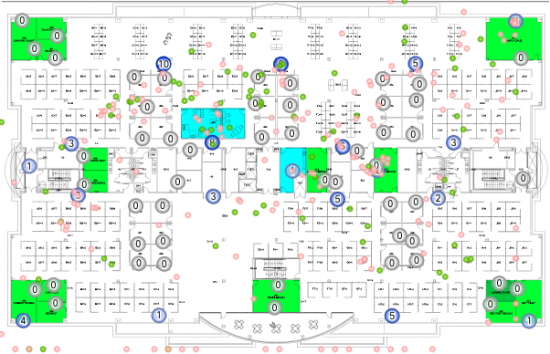
\includegraphics[scale=0.75]{cmx_map}
\caption{Positions of ~\acrlong{mu}s and which ~\acrlong{ap} they are connected to ~\cite{Shah2015a}}
\label{fig:toa}
\end{figure}
\subsection{CMX Engage}
\section{Location}
\subsection{Location Techniques}
\subsubsection{Proximity, Presence}
This technique is most feasible when dealing with outdoor positioning as it requires less \acrlong{ap}s but has less accuracy. According to the datasheet of Cisco \cite{Ciscoa}, the accuracy of this technique is limited to 10 to 30 metres. To calculate the user's position, the \acrshort{ap} with the strongest \acrlong{rssi} is picked as a correct representation of the \acrshort{mu}'s location.
\subsubsection{RSSI Triangulation}
\subsubsection{Hyperlocation}
\subsubsection{FastLocate}
\subsection{CMX Connect}
\subsection{CMX Analytics}
\section{Performance Metrics}
\subsection{Accuracy ~\& Precision}
\subsection{Coverage Area}
\subsection{Scalability}
According to documents provided by Cisco, most of the \acrshort{wlan} controllers are scalable with a decent throughput. Some statistics:
\begin{enumerate}
\item Cisco 5508: up to 500 \acrshort{ap}s and 7,000 clients are supported with a throughput of 8\acrfull{gbps}
\item Cisco 7510: up to 6,000 \acrshort{ap}s and 64,000 clients are supported with a throughput of 1\acrfull{gbps} in centrally switched traffic \footnote{All WLAN traffic is switched through a user-only WLAN network, meaning a locally switched WLAN can be active for employees without interfering with the user-only network. ~\cite{Woland}}
\end{enumerate}
There are numerous devices available that are not only dedicated to small or medium office, but also applicable to large multi-floor environments.
\subsection{Cost}
\subsection{Privacy}
\subsection{Conclusion}
\section{Conclusion}